\documentclass{beamer}
\usepackage{../common_slides}
\usepackage{tikz}
\usepackage{tikz-qtree}
\usepackage{pdfpages}

\title{Deep Learning and NLP}
\date{}
\author{CS 287}

\begin{document}
\begin{frame}
  \titlepage
\end{frame}


\begin{frame}{Foundational Challenge: Turing Test}
  \begin{quote}
    Q: Please write me a sonnet on the subject of the Forth Bridge.

    A : Count me out on this one. I never could write poetry.

    Q: Add 34957 to 70764.
    
    A: (Pause about 30 seconds and then give as answer) 105621.
    
    Q: Do you play chess?
    
    A: Yes.
    
    Q: I have K at my K1, and no other pieces. You have only K at K6 and R at R1. It is your move. What do you play?

    A: (After a pause of 15 seconds) R-R8 mate.
      {\normalfont - Turing (1950)}
  \end{quote}

\end{frame}

\begin{frame}{(1) Lexicons and Lexical Semantics}
  \textbf{Zipf' Law (1935,1949):}
  \begin{quote}
    The frequency of any word is inversely proportional to its rank in the frequency table.
  \end{quote}


     \begin{center}
       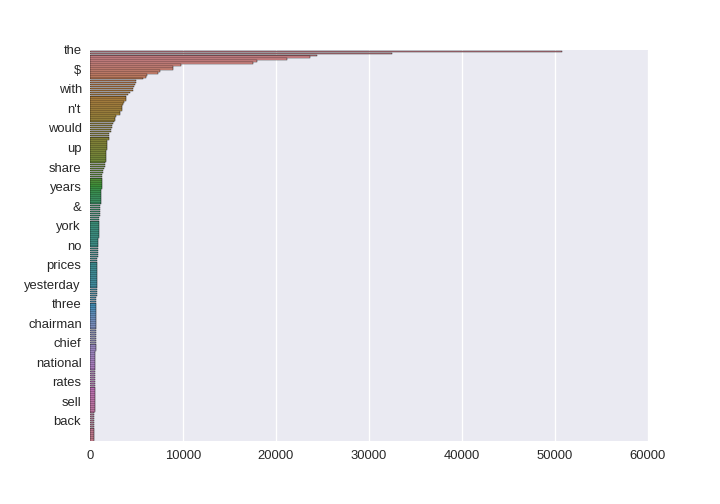
\includegraphics[width=0.8\textwidth]{../notebooks/zipf}         
     \end{center}
% \begin{itemize}
  % \item I.e. it is common to use rare words. 
  % \item Central issue in NLP is dealing cleverly with rare words. 
  % \end{itemize}
\end{frame}


\begin{frame}{(2) Structure and Probabilistic Modeling }
  \textbf{The Shannon Game (Shannon and Weaver, 1949):}
  \begin{quote}
    Given the last $n$ words, can we predict the next one?
  \end{quote} 
  

  \texttt{The pin-tailed snipe (Gallinago stenura) is a small stocky wader. It breeds in northern Russia and migrates to spend the \_\_ } 


  \begin{itemize}
  \item Probabilistic models have become very effective at this task.
  \item Crucial for speech recognition (Jelinek), OCR, automatic translations, etc. 
  \end{itemize}



\end{frame}

\begin{frame}{(3) Compositionality of Syntax and Semantics}
  \begin{quote}
    Probabilistic models give no insight into some of the basic
    problems of syntactic structure  {\normalfont - Chomsky (1956)}
  \end{quote}
  \begin{center}
    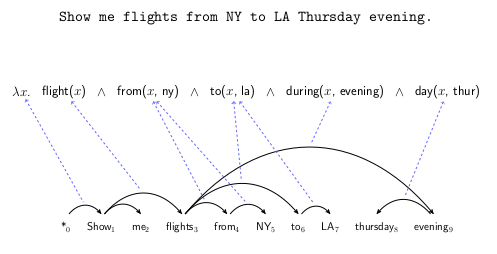
\includegraphics[width=10cm]{syntaxsem}
  \end{center}
\end{frame}


\begin{frame}{(4) Document Structure and Discourse}
  \begin{quote}
    Language is not merely a bag-of-words but a tool with particular
    properties  { - \normalfont Harris (1954)}
  \end{quote}
  \begin{center}
    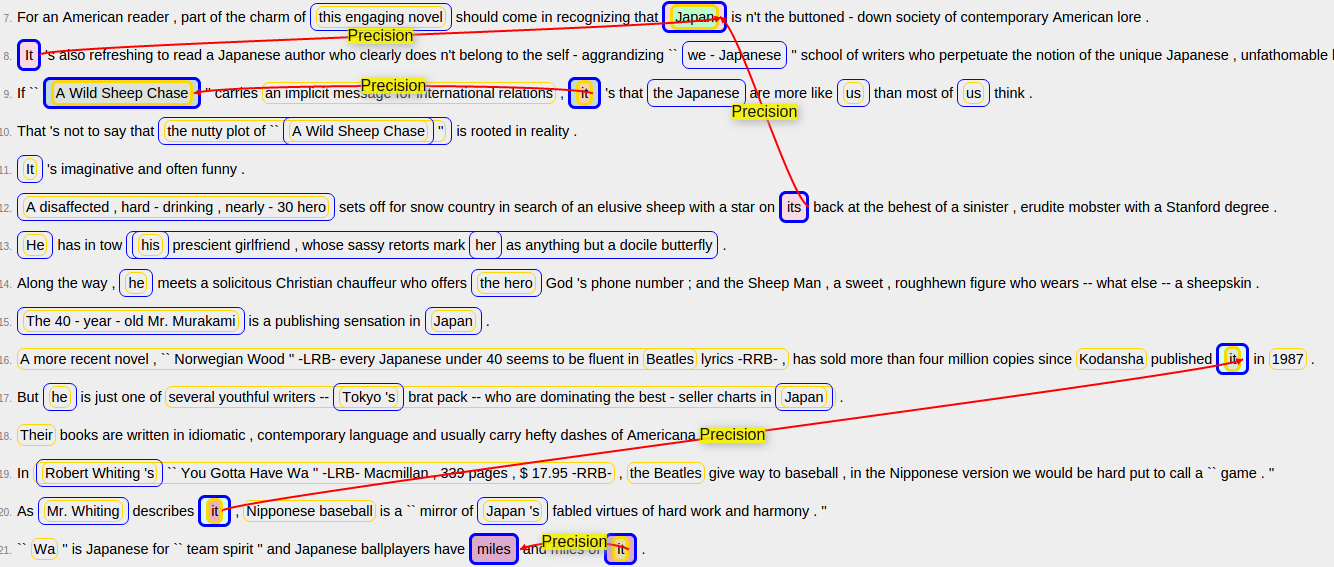
\includegraphics[width=\textwidth]{cort}
  \end{center}
\end{frame}

\begin{frame}{(5) Knowledge and Reasoning Beyond the Text}
\begin{quote}
It is based on the belief that in modeling language understanding, we must deal in an integrated way with all of the aspects of language — syntax, semantics, and inference. {- \normalfont Winograd (1972) }  
\end{quote}


\texttt{The city councilmen refused the demonstrators a permit because they [feared/advocated] violence.}


\begin{itemize}
\item Recently (2011) posed as a challenge for testing commonsense reasoning.  

\end{itemize}
\end{frame}


\section{Modeling}



\begin{frame}
  What have we covered? 
  \begin{itemize}
  \item $\boldx$; input representation
  \item $\boldy$; output representation 
  \end{itemize}
  Data-driven, end-to-end approach
\end{frame}

\begin{frame}{Input Representations}
  \begin{enumerate}
  \item Sparse Features
  \item Dense Features (Embeddings)
  \item Convolutional NN
  \item Recurrent NN
  \end{enumerate}
\end{frame}

\begin{frame}
  \begin{center}
    Which model should I use?
  \end{center}
  (No good general answer, but some rules of thumb...)
\end{frame}

\begin{frame}{Simple Classification}
\begin{verbatim}
  10 Mary moved to the hallway.
  11 Daniel travelled to the office.
  12 Where is Daniel?     office  11
\end{verbatim}

  Input is the sentences and the question, output is the answer
  \[ \mcC \] is set of possible answers 
\end{frame}



\begin{frame}{}
  ``Count-based Models''
  \begin{itemize}
  \item Naive Bayes, Kneser-Ney LM, HMM, 
  \end{itemize}

  \pause

  \begin{itemize}
  \item \structure{Fast to train, convex}
  \item \structure{Interpretable}
  \item \alert{Quite sensitive to features/independence assumptions}
  \item \alert{Need smoothing, overfitting hacks}
  \end{itemize}
\end{frame}

\begin{frame}
  Discriminative Linear models
  \air 

  \begin{itemize}
  \item Multiclass LR, windowed features, MEMM
  \end{itemize}
  \pause
  
  \begin{itemize}
  \item \structure{Convex}
  \item \structure{Somewhat interpretable}
  \item \alert{Sensitive to feature choice}
  \item \alert{Requires optimization to train}
  \end{itemize}
\end{frame}


\begin{frame}{Sparse Feature Approach}
  \begin{itemize}
  \item $p(y) p(x|y)$
  \end{itemize}
  \begin{itemize}
  \item $p(y)$ prior on answers
  \item $p(x|y)$ determined by feature set.  
  \end{itemize}
\end{frame}

\begin{frame}{Pipeline Sparse Feature Approach}

\begin{verbatim}
  11 [Daniel] travelled to the [office].
  12 Where is [Daniel]?     office  11
\end{verbatim}

  \begin{enumerate}
  \item Run tagging to POS tags.
  \item Run NER to find named entities.
  \item Run parsing to find syntax.
  \item Construct Features from this data i.e. 
    Mary  
    
  \end{enumerate}

\end{frame}

\begin{frame}{Stanford CoreNLP}
  
\end{frame}


\begin{frame}
  Shallow feed-forward neural networks
  \air 

  \begin{itemize}
  \item Windowed NN, CBoW Embeddings, Bengio NNLM, NN-MEMM
  \end{itemize}
  \paurse

  \begin{itemize}
  \item \structure{Learn feature combinations end-to-end}
  \item \structure{Improved performance on several tasks}
  \item \alert{Non-convex}
  \item \alert{Requires large amount of (semi-)supervision}
  \item \alert{Sensitive to hyper-parameters}
  \end{itemize}
\end{frame}

\begin{frame}{End-to-End Simple Approach}

\begin{verbatim}
  11 [Daniel] travelled to the [office].
  12 Where is [Daniel]?     office  11
\end{verbatim}

  \begin{enumerate}
  \item Use CBoW or convolution to construct word representation 
  \item Use  
  \item Train end-to-end
  \end{enumerate}

\end{frame}


\begin{frame}
  Recurrent neural networks
jj  \begin{itemize}
  \item RNN/GRU/LSTM, acceptor, transducer, encoder-decoder
  \end{itemize}

  \begin{itemize}
  \item \structure{Learn feature combinations end-to-end}
  \item \structure{Learn sequence representation (!) end-to-end}
  \item \structure{Improved performance of sequence modeling tasks}
  \item \alert{Non-convex, and sensitive to exploding/vanishing gradient}
  \item \alert{Requires large amount of (semi-)supervision}
  \item \alert{Sensitive to training, hyper-parameters, model size}
  \item Requires greedy/beam search (non-Markovian)
  \end{itemize}
\end{frame}

\begin{frame}
\begin{verbatim}
  11 [Daniel] travelled to the [office].
  12 Where is [Daniel]?     office  11
\end{verbatim}

  \begin{enumerate}
  \item Use RNN to construct representation
  \item Train end-to-end
  \end{enumerate}
\end{frame}

\begin{frame}
  Questions to ask: 
  \begin{itemize}
  \item Do I have significant amounts of supervised data?
  \item Do I have prior knowledge of my problem/domain?
  \item What is the underlying metric of interest?
  \item Do I need interpretability of the model? 
  \item Is the structure of the text important?
  \item Is training efficiency/prediction efficiency important?
  \end{itemize}
\end{frame}

\begin{frame}{Loss Functions}
  \begin{itemize}
  \item Generative $p(x, y)$
    \begin{itemize}
    \item Maximum Likelihood
    \item Smoothing
    \end{itemize}
  \item Discriminative $p(y | x)$
    \begin{itemize}
    \item Cross-Entropy 
     \item Hinge Loss
    \end{itemize}
  \end{itemize}
\end{frame}


{
\setbeamercolor{background canvas}{bg=}
\includepdf[pages=19]{slides_wpi.pdf}
}



\begin{frame}{Output Representations}
  \begin{enumerate}
  \item Ranking (score the output)
  \item Simple Multiclass Output
  \item Large Multiclass Output (HSM, NCE) 
  \item Structured (sequence)
  \end{enumerate}
\end{frame}


\begin{frame}{Search}
  \begin{enumerate}
  \item Multiclass Prediction
  \item Greedy Search
  \item Beam Search
  \item Viterbi Search
  \end{enumerate}
\end{frame}

\begin{frame}{Tasks}
  \begin{itemize}
  \item Text Classification 
  \item Part-of-Speech Tagging
  \item Language Modeling
  \item Sequence Modeling
  \item Named-Entity Recognition
  \end{itemize}
\end{frame}

\section{AlphaGo}

\begin{frame}
  
\end{frame}

\begin{frame}{Simple Idea: Greedy Player}
  
\end{frame}


\begin{frame}
  $\hat{\boldy}$ distribution over next move  
\end{frame}

\begin{frame}{Data-Driven Player}
  Dataset move  .. .
  
  Pretty big data set... 
\end{frame}

\begin{frame}{Image}
  
\end{frame}

\begin{frame}{Move}
  
\end{frame}


\begin{frame}{Classical Tree Search}
  
\end{frame}

\begin{frame}{Depth-Limited Tree Search}
  
\end{frame}


\begin{frame}{Heuristic State Evaluation}
  
\end{frame}

\begin{frame}{Train on Data}
  
\end{frame}


\begin{frame}{Roll-Out}
  
\end{frame}

\begin{frame}{How do you compute this heuristic?}
  
\end{frame}

\begin{frame}{Learning Better Heuristic}
  \begin{itemize}
  \item Play game against itself
  \item 
  \end{itemize}
\end{frame}

\begin{frame}{Monte Carlo Tree Search}
  
\end{frame}

\begin{frame}
  
\end{frame}

\begin{frame}
  
\end{frame}

\end{document}